\documentclass{article}
\usepackage{natbib}
\usepackage{graphicx}
\usepackage[english]{babel}
\usepackage[utf8]{inputenc}
\usepackage{url}
\usepackage{fancyhdr}
\pagestyle{fancy}
\fancyhf{}
\rhead{CSI5155-Machine Learning}
\lhead{University of Ottawa}
\rfoot{Page \thepage}

\begin{document}

\section*{CSI\_5155\_Project\_Proposal\_Group\_7}

\begin{itemize}
\item Project Title: Understanding the Words of Deaf-mute People by Machine Learning Based Gesture Recognition
\item Project Type: application oriented
\item Names of Group Members: Lingfeng Zhang,300134245; Biliang Wang,300105002
\item Description of the Dataset: 
    \begin{itemize}
        \item Dataset Name: ASL Alphabet: Image data set for alphabets in the American Sign Language
        \item Available Link: \newline \url{https://www.kaggle.com/grassknoted/asl-alphabet}
        \item Detailed Illustration: 
        \item Dataset Size: 87,000 images which are 200$\times$200 pixels, so this dataset has 87,000 rows and each datum has 200$\times$200 features. We can resize the images to reduce the feature numbers later.
        \item Classification: 29 classes, of which 26 are for the letters A-Z and 3 classes for SPACE, DELETE and NOTHING. Part of these classes is shown in Figure \ref{fig:hands}
    \end{itemize}
    	\begin{figure}[h!]
        \centering
        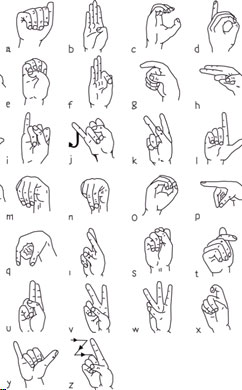
\includegraphics[scale=0.7]{NIDCD-ASL-hands-2014.jpg}
        \caption{Representation of Gestures}
        \label{fig:hands}
        \end{figure}
\item Project Description: In this project, we plan to classify hand gesture pictures into 29 classes to help understand the words of deaf-mute people. We will use tree-based, rule-based and distance-based methods, as well as linear models to classify these pictures and analyze the difference of accuracy and other differences between these different machine learning models. In addition, we will analyze the pros and cons of these different machine learning models according to researching the algorithms or the processing of classification methods. Finally, we hope we can apply the best of these machine learning models to recognize the hand gesture, trying to enable the model to illustrate the meanings of different hand gestures with high accuracy as much as possible. If we find a better state-of-art machine learning method to recognize hand gesture, we will illustrate it too. The reason why we are interested in hand gesture recognition is that this field can also be applied in games, unlocking smartphones and so forth besides automated sign language translation.
\item Statement: I hereby certify I will not use
these dataset(s) and algorithm(s) in any other courses, past, present or future. I understand that submitting overlapping material for more than one course is not allowed. This work is also not part of my thesis or capstone project research. I understand that any such action on my part will lead to a grade of INC being awarded for CSI5155 and may lead to academic sanctions imposed by the faculty of Engineering.
\end{itemize}

\end{document}
